\chapter{Measurement of Neutral Current Quasielastic
Interactions with Super-Kamiokande Gadolinium Upgrade}
\label{chp:ncqegd}

\section{Event Simulation}

This chapter discusses details about the event simulation, specifically the software used and the way neutrino interactions are simulated in order to produce Monte Carlo. Table \ref{table:software} summarises all the software used in this analysis. 


\begin{table}
$$
\begin{array}{ll}
\hline \text { Name } & \text { Version } \\
\hline \text { Flux } & 13 \text { a tuning v4.0 } \\
\text { NEUT } & 5.3 .3 \\
\text { SKDETSIM-SKGd } & \text { ANNRI-Gd model } \\
\text { Geant } & 4.10.05.p01 \\
\text { T2KReWeight } & \text { v1r23 } \\
\text { GENIE } & \text { R2-12-10 } \\
\hline
\end{array}
$$
\end{table}

\subsection{Neutrino flux}

The neutrino beam flux used in this analysis is 13a tuning v4.0, taken from the NA61/SHINE fixed target experiment at CERN \cite{vladisavljevic_constraining_2018}.  The NA61/SHINE experiment provides hadron production measurements for T2K and other long baseline experiments, and measures the yield of charged hadrons from a proton beam fired at a thin graphite target (2 cm long) and a T2K replica graphite target (90 cm long). From this experimental data, Monte Carlo simulations of the neutrino flux are predicted. The oscillation effect on the neutrino flux needs to be considered after choosing which flux to use, and although the neutrino-oxygen NCQE cross section does not depend on flavour (and therefore neutrino oscillation affects would have no impact on a fully pure NCQE sample) there is a small amount of charged current events which seep into the NCQE sample, and oscillation weights need to be applied to the charged current events in the sample. Monte Carlo reweighting takes care of this issue by assuming that they are all muon neutrino or muon anti-neutrino events, due to the fact that the number of electron neutrino events in FHC mode would be negligible.

\subsection{Primary interaction}

The interaction between the incoming neutrino event and an Oxygen nucleus, and it's consequent de-excitation is modelled by NEUT, which produces a vector of primary particles. Because these are primary particles, they do not take into consideration all the particles produced from the detector response, i.e. the secondary particles produced from the interactions within the medium of the detector, in our case, water doped with gadolinium sulphate octahydrate. The way NEUT treats the interaction between a nucleus and a neutrino for the case of a neutrino interaction with a $16_{O}$ isotope is shown in Equation \ref{eq:neutrinonuc}. 

\begin{equation}
    \sigma\left(\nu^{16} \mathrm{O}\right)=\sum_{i=1}^{8} \sigma_{\mathrm{p}}\left(p_{i}^{(\mathrm{p})}\right)+\sum_{j=1}^{8} \sigma_{\mathrm{n}}\left(p_{j}^{(\mathrm{n})}\right)+\sigma(2 p 2 h)    
\label{eq:neutrinonuc}    
\end{equation}

Here $\sigma_{p}$ and $\sigma_{n}$ are the neutrino-proton cross section and the neutrino-neutron cross section respectively, and these cross-sections are dependent on the momenta of the protons and neutrons in the model, and therefore on the choice on nuclear model. The Benhar Spectral Function (SF) is used by NEUT as the nuclear model for NCQE interactions, and for CCQE interactions the Smith-Moniz relativistic Fermi Gas (RFG) model is used \cite{benhar_electron-_2005}, with 2p2h interactions included for these interactions. 

\begin{figure}
    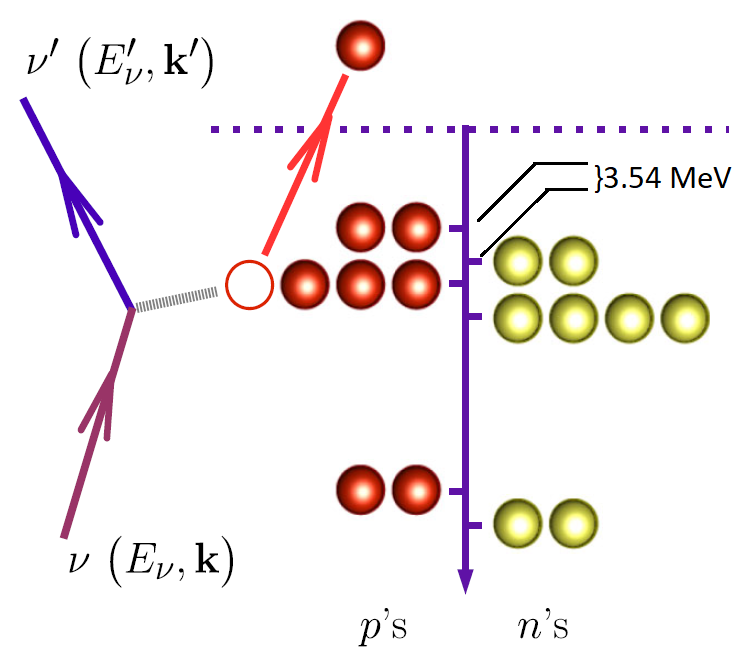
\includegraphics[width=\textwidth]{Figures/ncqebenharspectral.png}
    \caption{Representation of NC neutrino scattering off $16_{O}$ with protons on the left hand side and neutrons on the right arranged according to the shell model. }
    \label{fig:ncqebenharspectral}
\end{figure}

The lowest rung of nucleons in Figure \ref{ncqebenharspectral} is the $s_{1/2}$, with $p_{3/2}$ above this level and $p_{1/2}$ above that. The protons in these rungs have removal energies of 12.1 MeV, 18.4 MeV and 42 MeV respectively, and due to neutron levels being more tightly bound, these have an extra removal of 3.24 MeV compared to their proton counterparts. The shell model is imperfect due to how it allocates the probablity of $16_{O}$ transitioning to the possible nucleon states. In the shell model, probabilities are allocated by counting the number of nucleons in each energy level and assigning probailities according to how many there are. In Figure \ref{fig:ncqebenharspectral} it can be seen that the $p_{3/2}$ state has double the number of nucleons compared to the $s_{1/2}$ model and therefore double the probability of transition is assigned for the $p_{3/2}$ state, and the probability of transitioning to any other state is assigned to be 0, because in the shell model they don't even exist. The Benhar Spectral Function model however is complex and is tuned using electron-nucleus scattering data. The model used in this analysis is a modified version of the Benhar Spectral Function model, where the case of other transition states is dealt with by merging the "others'' state into the $s_{1/2}$ state. Table \ref{table:transitionprob} gives the probabilities of transition to different states for different models. 

\begin{table}
$$
\begin{array}{ccccc}
\hline & \left(\mathrm{s}_{1 / 2}\right)^{-1} & \left(\mathrm{p}_{3 / 2}\right)^{-1} & \left(\mathrm{p}_{1 / 2}\right)^{-1} & \text { others } \\
\hline \text { Shell model } & 0.25 & 0.5 & 0.25 & 0 \\
\text { Spectral Function } & 0.1055 & 0.3515 & 0.158 & 0.385 \\
\text { This analysis } & 0.4905 & 0.3515 & 0.158 & 0 \\
\hline
\end{array}
$$
\label{Transition probabilities for different models and states}
\end{table}

\subsection{Detector response and interactions in the detector medium}

Prior analyses to this used SKDETSIM (Super-Kamiokande Detector Simulator) to simulate the trajectories of particles through the water in Super-Kamiokande and output detector response MC. This analysis uses SKDETSIM-SKGd to propogate the particles




\section{Event Reconstruction}
\subsection{Bonsai output reconstruction quantities}

Due to this analysis looking specifically at the low energy region, a fitter specific to low energies (called LOWFIT) is used to reconstruct events. Both MC and data neutrino events undergo a reconstruction phase, where the low-energy fitter BONSAI is applied to the event, which is discussed in Chapter 2. This reconstruction is carried out using timing and cable information, however charge information is omitted. The ouput of BONSAI gives information which will be used in the reduction phase of the data and allow for the selection of the NCQE sample. The following quantities comprise the BONSAI output, the first two being helpful spectator variables and the latter five constituting parameters which are used in the reduction phase of the analysis, from which the neutrino NCQE sample is determined.\\

\underline{Neutrino vertex direction}\\

This vector points towards the direction which is an average over all the Cherenkov cone axes which are produced, due to there being multiple leptons induced in the interaction.\\



\underline{Neutrino vertex position}\\
The reconstructed location of the neutrino interaction event.


 \underline{Reconstructed energy}\\
 In line with the standard SK low energy analysis definition, this energy is simply the reconstructed energy with the 0.511 MeV electron mass omitted. The range for Erec in this variable is 3.49 MeV to 29.49 MeV - the estimated kinetic energy under the hypothesis that the event is a singular electron.
\newline

 \underline{Dwall}\\
 This variable gives the minimum distance of the neutrino vertex position from the closest wall of the Super-Kamiokande detector.
\newline

 \underline{Effwall}\\
 Thus variable gives the distance between the neutrino vertex posiiton and the closest wall, but moving back from the vertex position along the neutrino vertex direction vector.
\newline

 \underline{Vertex direction and goodness coefficient}\\
 The coefficient $ovaQ$ (defined in Equation \ref{ovaq}) describes the quality of the vertex reconstruction. It consists of two parameters $g^2_{vtx}$ and $g^2_{dir}$ where the former describes the goodness of the vertex which is based on PMT hit timings, and increases the sharper an event is in time. The latter is the directional goodness and measures the azimuthal uniformity in the ring pattern produced by the Cherenkov cone, which decreases the more uniform an event is in space. As a result of this, $ovaQ$ increases the more uniform and sharp in time an event is.

\begin{equation}
    \text { ova } Q=g_{\text {vtx }}^{2}-g_{\text {dir }}^{2}
    \label{ovaq}
\end{equation}

$g_{vtx}$ is calculated using a fit of the PMT timing distribution and using the hit times of the PMT it is defined asin Equation\ref{vertex_goodness}.

\begin{equation}
g_{\mathrm{vtx}}=\frac{\sum_{i} w_{i} \mathrm{e}^{-\frac{1}{2}(\frac{\Delta t_{i}}{\sigma})^{2}}}{\sum_{i} w_{i}} \text { with } w_{i}=-\frac{1}{2}(\frac{\Delta t_{i}}{\omega})^{2}
\label{vertex_goodness}
\end{equation}

Here $\sum_{i} w_{i}$ is the weight given to the i-th hit PMT for the reduction of dark noise, where $\omega$ has a value of 60ns. $\sigma$ has a value of 5ns which is used to test the goodness, and as a result, a sharp timing distribution produces a large vertex goodness. $g_{dir}$ is calculated by looking at how spatially uniform the hit PMTs are around the reconstructed neutrino vertex direction. In order to quantify this uniformity, the Kolmogorov-Smirnov (KS) test is used as in Equation \ref{direction_goodness}.

\begin{equation}
    \mathrm{g}_{\mathrm{dir}}=\frac{\max _{i}\{\angle_{\mathrm{uni}}(i)-\angle_{\mathrm{data}}(i)\}-\min _{i}\{\angle_{\mathrm{uni}}(i)-\angle_{\mathrm{data}}(i)\}}{2 \pi}
\label{direction_goodness}
\end{equation}

where $\angle_{\mathrm{data}}(i)$ is the azimuthal angle of i-th hit real PMT included in the number of hits in 50ns. $\angle_{\mathrm{uni}}(i)=2 \pi i / N_{50}$ is the azimuthal angle of the i-th virtual PMT hit, but only when uniform distribution of the hits is assumed. As the uniformity of the hit pattern increases, the goodness decreases. 
 



 \underline{Cherenkov angle $theta_{C}$}

 For relativistic electrons in water, the value of the Cherenkov opening angle is $\approx 41\degree$, due to the relation: 

 \begin{equation}
\cos \theta_{\mathrm{Cherenkov}}=\frac{1}{n\beta}
\label{cherenkov_angle}
\end{equation}
 
where $\beta = v/c \approx 1$ and $n$ is the refractive index of water, 1.33. However due to other particles in the simulation, such as protons or muons, the Cherenkov cone is expected to be narrower, or if multiple leptons are present, the Cherenkov cones will be less distinct and more spread out, leading to deviations from the 41\degree value. 


\subsection{True neutron tagging information}
\subsection{Primary selection criteria}
\subsection{Secondary selection criteria}
When the neutron vertex is found by this method, 14 variables which describe different aspects of the neutron candidate are calculated. For each of the neutron candidates the vector of these variables are computed and fed into the neural network and this produces an output value which is between 0 and 1. These variables relate to different features regarding categorising hits from neutron capture on Gd or H, including the number of the hits from neutron capture, the isotropy of these hits, the Cherenkov angles of these hits and the position of the neutron vertex in the detector when capture occurs. A description of these variables are given as follows:


\underline{N10nvx}
\newline
This is the number of hits in the 10ns sliding window of the neutron candidate
\newline


\underline{N300S}
\newline
Excluding the number of hits in the 10ns sliding window (N10nvx), this is the number of hits in the extended window of 300ns.
\newline


\underline{NcS}
\newline
This variable is defined as:
\begin{equation}
\label{ncs}
    NcS = N10nvx - Nclushit
\end{equation}

    Where $Nclushit$ is the number of clusterised hits: if hit \textit{i} and \textit{j} are hits on PMTs, then for hit \textit{i} and hit \textit{j} the hit vector $\hat{r}_i$ can be written as:

\begin{equation}
\label{hit}
    \hat{r}_{i}=\frac{\overrightarrow{P M T_{i}}-\overrightarrow{V T X_{n}}}{\left\|\overrightarrow{P M T_{i}}-\overrightarrow{V T X_{n}}\right\|}
\end{equation}

where the angle at the point of the neutron capture vertex between $\hat{r}_{i}$ and $\hat{r}_{j}$ of the PMT hits is defined as:

\begin{equation}
\theta_{i j}=\arccos \left(\hat{p}_{i} \cdot \hat{p}_{j}\right)
\end{equation}

where the hits are defined as clustered if $\theta_{ij}$ is less than 14


\underline{llrca}
\newline
This variable is the log likelihood ratio calculated using triplets of hits from N10nvx that make up a rudimentary Cherenkov cone, from which the opening angle $\theta$ is calculated. Two PDFs ($\theta_{Ci}$) and ($\theta_{Ci}$) are calculated from each $\theta_{Ci}$ where p\_s and p\_b are the probability density functions of $\theta_{C}$ depending on whether the hits come from a true neutron capture on Gd or H or a false neutron capture which makes up the background. The log likelihood ratio variable is computed using Equation {\ref{llrca}}.

\begin{equation}
\label{llrca}
\newline
  llrca =\sum_{i \in\{ { triplets }\}} \log \left(\frac{f_{B}\left(\theta_{C i}\right)}{f_{S}\left(\theta_{C i}\right)}\right)
\end{equation}


\underline{beta-n}
\newline
These variables (where n = 1,2,3,4,5) are defined using Legendre polynomials, shown in Equation \ref{beta}, which gives the isotropy of the Cherenkov hits.

\begin{equation}
\label{beta}
 beta- n=\frac{2}{N 10 {nvx}(N 10 {nvx}-1)} \sum_{i \neq j}  { Legendre }_{n}\left(\cos \theta_{i j}\right)
\end{equation}

where $Legendre_n$ gives the Legendre polynomial of order $n$ and $theta_{ij}$ is the angle between hit PMTs relative to the neutron capture vertex.



\underline{ndwall}
\newline
This parameter, similar to dwall, gives the shortest distance of the neutron capture vertex from the wall of the Super-Kamiokande tank.
\newline



\underline{ntowall}
\newline
This variable (similar to effwall), gives the distance of the neutron capture vertex from the wall, however, unlike ndwall it gives the direction of the neutron capture specifically along the direction of the centre of the hits. The direction ($\overrightarrow{R}$) is given by:

\begin{equation}
\overrightarrow{\operatorname{dir}}=\sum_{i=1}^{N 10 n v x} \hat{p}_{i}
\end{equation}





